\documentclass[10pt, a4paper, oneside, titlepage]{scrartcl} % article hat kein subtitle
\usepackage[utf8]{inputenc}
\usepackage{mathpazo}
\usepackage{setspace}
\usepackage{lscape}
\setstretch{1.3}
\usepackage{fancyhdr}
\pagestyle{fancyplain}
\fancyhead{}
\chead{\textbf{\leftmark{}}}
\cfoot{}
\rfoot{ \thepage{}  / \pageref{letzte_seite}}
\renewcommand{\headrulewidth}{0.8pt}
\usepackage{sectsty}
\sectionfont{\hspace{10pt}}
\subsectionfont{\vspace{30pt}}
\subsubsectionfont{\vspace{30pt}}
\usepackage[labelsep=colon, font=small, labelfont=bf]{caption}
\usepackage[pdftex]{graphicx}
\usepackage[pdftex]{color}
\usepackage{colortbl}
\usepackage{parskip}
\usepackage[ngerman]{babel}
\usepackage{longtable}
\date{2. Dezember 2013}
\hyphenation{Auf-sichts-rat Com-piler}
\author{Björn Ahlfeld, Patrick Borck, Jens Grundmann,\\ Sebastian Lun, Daniel Pinkpank, Phillippe Wels}
\title{LIAR - Lügendetektor}
\subtitle{Semesterprojekt im Fach Mobile Applications for Public Health}
\frenchspacing{} 
%-------------------------------------------------------------------
\begin{document}
   	\maketitle
   	\thispagestyle{empty}
	\tableofcontents
	\listoffigures
	\listoftables
   	\newpage
   	\section{Projektplanung}  
   \begin{figure}[ht!]
	\begin{center}
		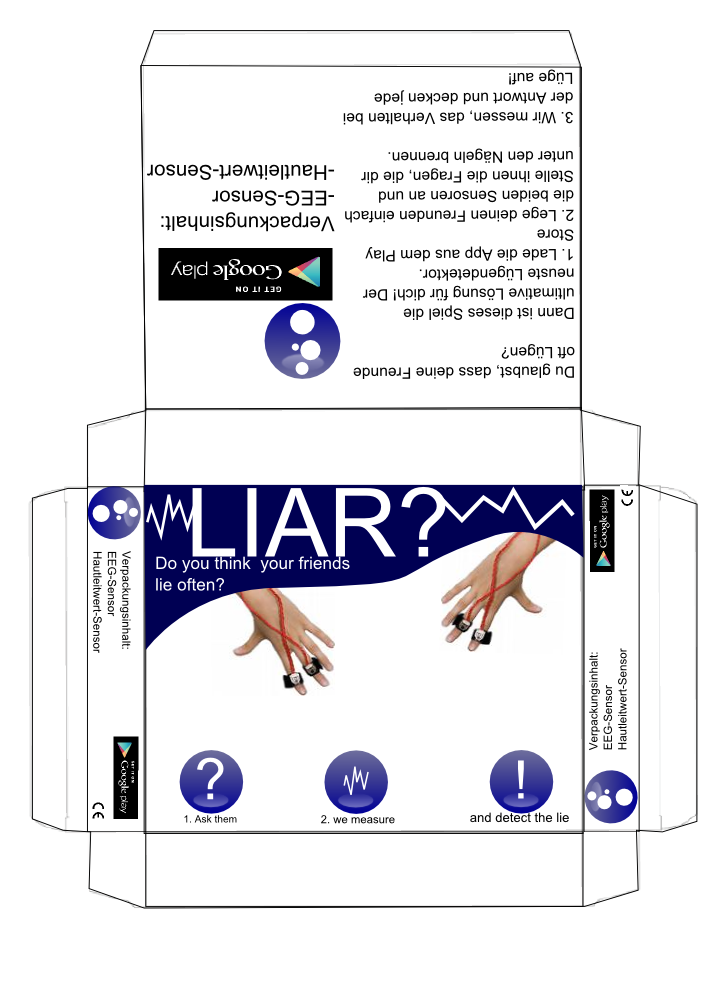
\includegraphics[scale=0.5]{verpackung_bjoern.png}
	\end{center}
	\caption[Produktverpackung]{Produktverpackung Liar Android App}
	\label{fig:verpackung}
	\end{figure}

	\newpage
	\section{Fiktive Zeitungsmeldung}
		
	\begin{figure}[hbtp]
	\begin{center}	
	\begin{minipage}[t]{0,8\textwidth}
			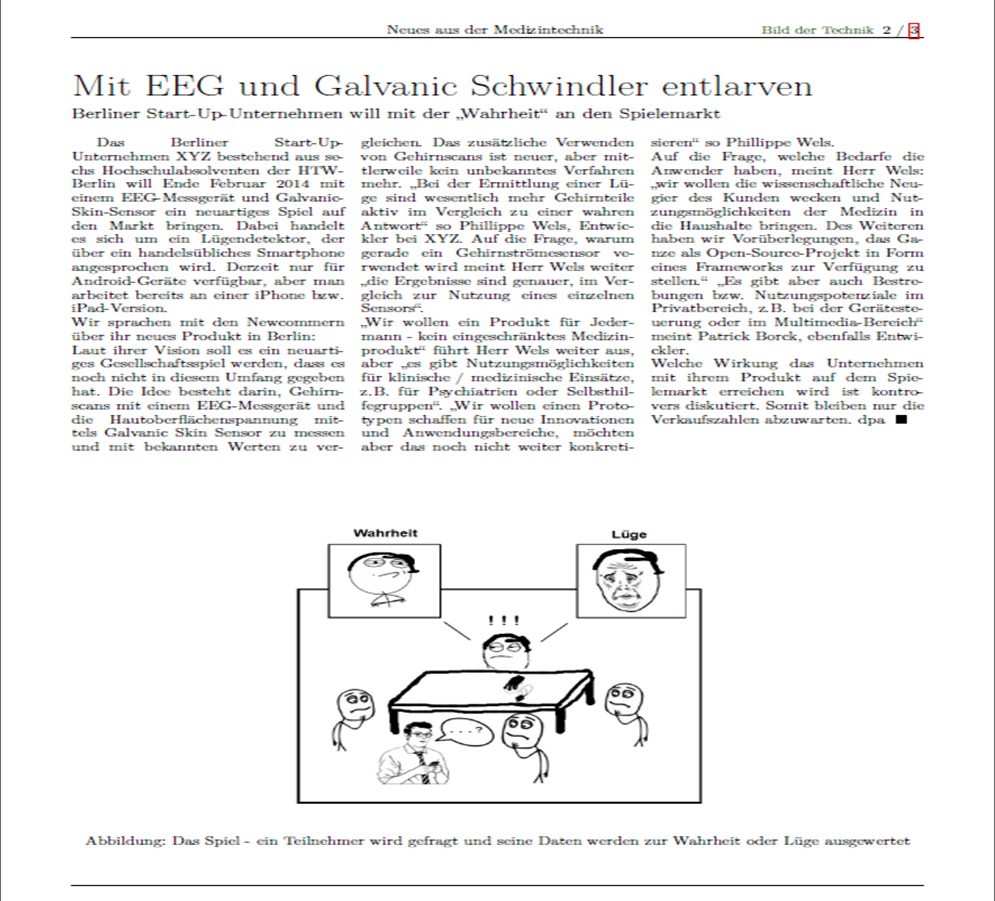
\includegraphics[scale=0.63]{zeitungsmeldung_bild.png}
	\end{minipage}
	\end{center}	
	\caption[Zeitungsmeldung]{Zeitungsmeldung zum Lügendetektor}
	\label{fig:zeitung}
	\end{figure}
	
			
	\begin{figure}[ht!]
	\begin{center}
		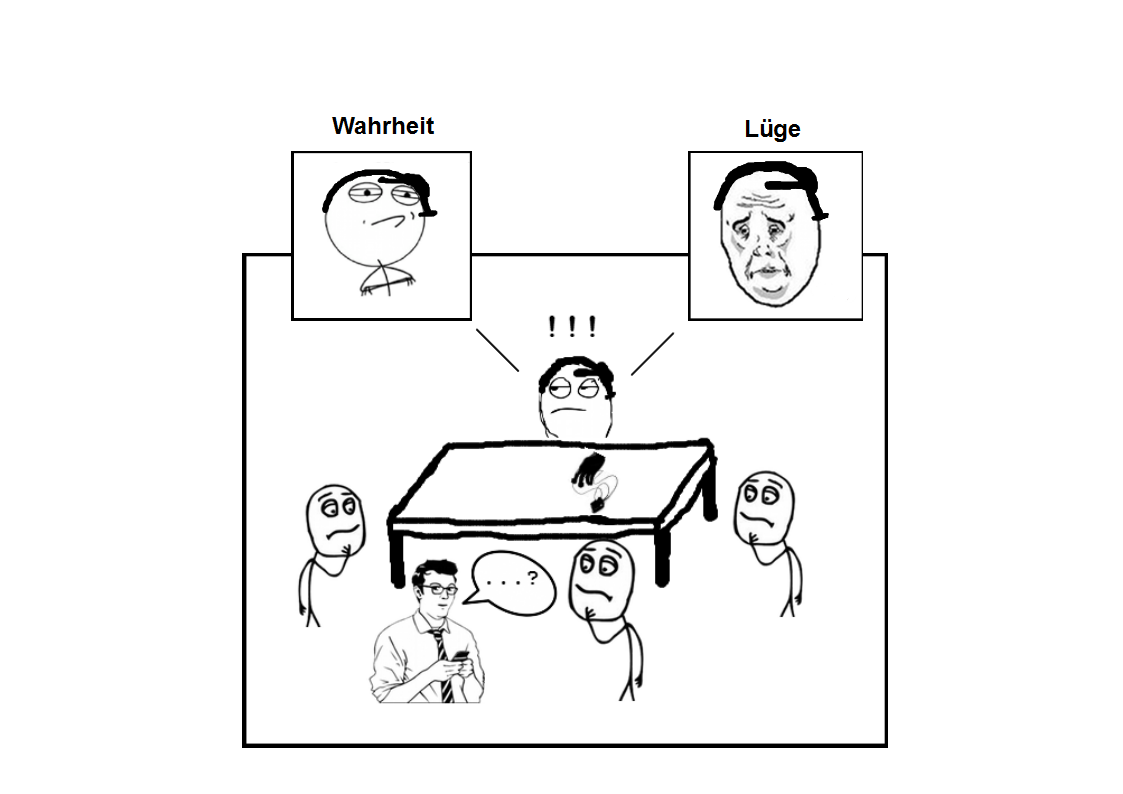
\includegraphics[scale=0.45]{SessionImg.png}
	\end{center}	
	\caption[Das Spiel]{Grundidee des Lügendetektorspiels}
	\label{fig:session}
	\end{figure}
	
	\newpage
 
	\section{Meilensteine, Arbeitsaufteilung}
   
   	\section{Personas, Anwendungsszenarien}
   	Eine Persona stellt einen Prototyp für eine Gruppe von Nutzern dar, mit konkret ausgeprägten Eigenschaften und einem konkreten Nutzungsverhalten.
   	
	\subsection{Elissa Schubert (20)}
	\begin{center}
		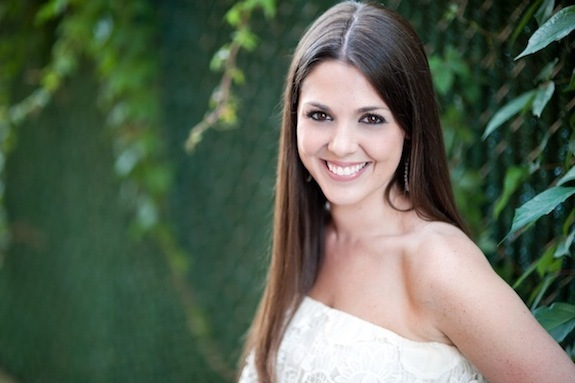
\includegraphics[width=10.0cm]{persona_01.jpg}
	\end{center}
	\begin{itemize}
		\item{}studiert Deutsch und Biologie auf Lehramt an der Universität zu Köln.
		\item{}singt im Chor, geht gern auf Partys und engagiert sich beim WWF.
		\item{}ist notorisch eifersüchtig auf jede Frau, die sich Ihrer Jugendliebe Bernd nähert. Da Bernd auch dafür bekannt ist, mehrgleisig unterwegs zu sein, 		will sie Gewissheit, dass er nur sie liebt.
		\item{}will mit Bernd eine Familie gründen und erfolgreich Ihr Studium beenden.
		\item{}mag es nicht belogen zu werden. Sie ist ein Kontrollfreak und liest heimlich die SMS von Bernd.
	\end{itemize}	   
   
   	\subsection{Frank Bollwerker (36)}
   	\begin{center}
		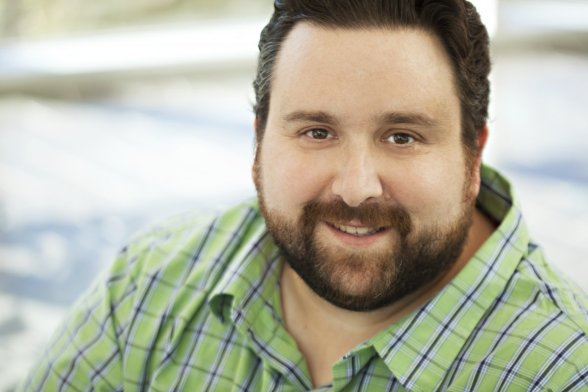
\includegraphics[width=10.0cm]{persona_02.jpg}
	\end{center}
	\begin{itemize}
		\item{}arbeitet als wissenschaftler Mitarbeiter im Studiengang Luft- und Raumfahrttechnik an der Universität Stuttgart.
		\item{}ist verheiratet und zur Zeit noch kinderlos. 
		\item{}spielt in seiner Freizeit Basketball und geht gerne Wandern.
		\item{}ist in der Themenfindung für seine Doktorarbeit und möchte erweiterte Tests zur Auswahl der zukünftigen Raumfahrer entwickeln. Er sucht dabei eine 		Möglichkeit seine schriftlichen Tests zu validieren.
	\end{itemize}		

	\subsection{Jonas Keppler (29)}
	\begin{center}
		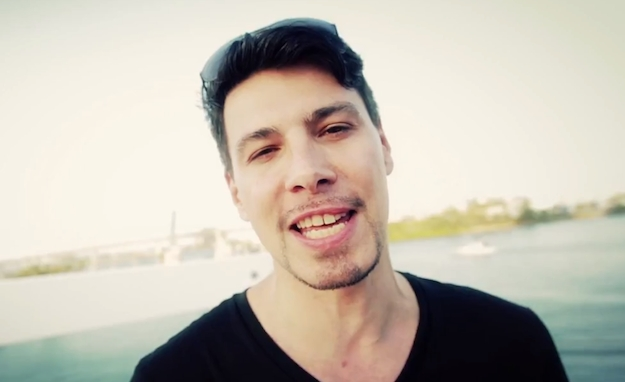
\includegraphics[width=10.0cm]{persona_03.jpg}
	\end{center}
	\begin{itemize}
		\item{}arbeitet als Redakteur im Ressort "Digital" bei der Süddeutschen Zeitung in München.
		\item{}ist sehr interessiert an neuer Technik und coolen Apps, die er dann stolz während der Mittagspause all seinen Arbeitskollegen präsentiert. Er 				steht gern im Mittelpunkt.
		\item{}geht gern ins Kino und schaut sich jeden Donnerstag die Sneak Preview an, um mitreden zu können.
		\item{}macht Yoga und achtet sehr auf seine Ernährung.
		\item{}kauft im Biomarkt ein und wird im nächsten Sommer erstmals selbst Gemüse auf seinem Grundstück anbauen.
	\end{itemize}
	
   	\section{Anforderungen (priorisierte User Stories)}

	\begin{landscape}
   	\section{Risikobetrachtung}
   	\begin{table}[h!]
		\begin{center}
			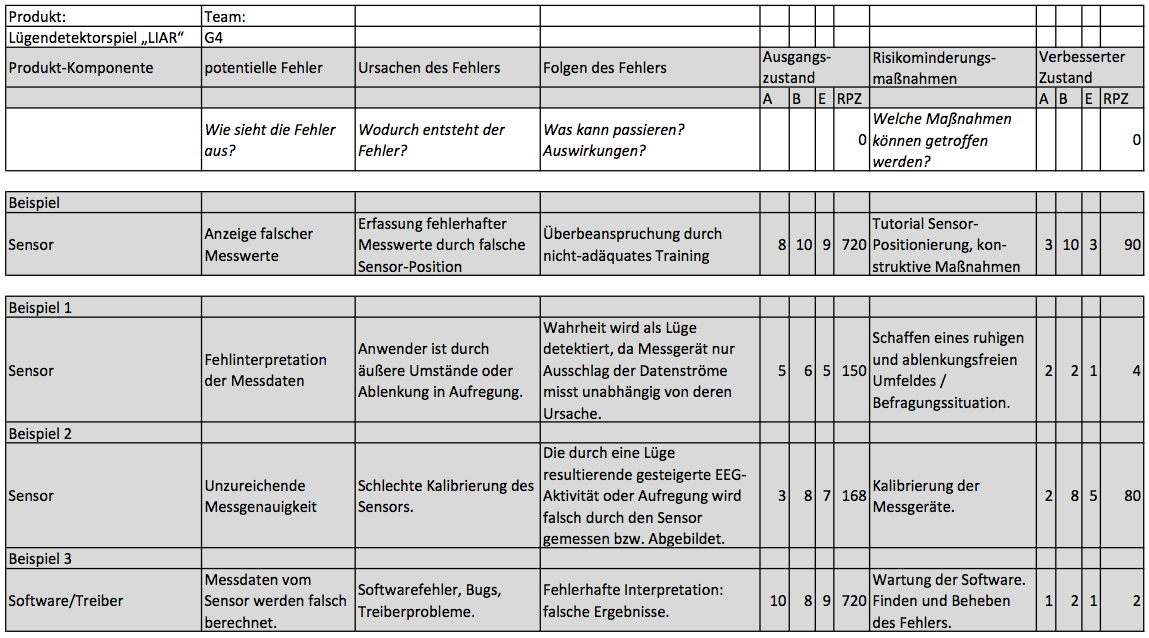
\includegraphics[scale=0.45]{Risikobetrachtung.png}
		\end{center}
		\caption[Risikoanalyse]{Risikoanalyse}
		\label{fig:risikoanalyse}
	\end{table}
	\end{landscape}
   
   \section{Systemüberblick, Architektur}
   \section{Entwurf / Mock-up User-Interface}

\label{letzte_seite} % zum Seiten zählen
\end{document}
